\documentclass{article}

%--------------------------------------------------------------
% Document & Font Setup
%--------------------------------------------------------------
\usepackage[a4paper, margin=1in]{geometry}
\usepackage{setspace}
\usepackage{parskip}
%--------------------------------------------------------------
% Common Packages
%--------------------------------------------------------------
\usepackage{graphicx}
\usepackage{subcaption}
\usepackage{caption}
% Subfigure captions
\DeclareCaptionLabelFormat{custom}{\figurename~\thefigure~(#2)}
\captionsetup[subfigure]{labelformat=custom}

\usepackage{enumitem}
\usepackage{float}
\usepackage{placeins}
\usepackage[dvipsnames,x11names,svgnames]{xcolor}
\usepackage{url}

%--------------------------------------------------------------
% Math & Science Packages
%--------------------------------------------------------------
\usepackage{amsmath,amssymb,amsfonts,amsthm}
\usepackage{mathtools}
\usepackage{bbm}
\usepackage{siunitx}
\DeclareSIUnit{\rpm}{RPM}
\DeclareSIUnit{\au}{AU}

%--------------------------------------------------------------
% Hyperlinks
%--------------------------------------------------------------
\usepackage{hyperref}
\hypersetup{
    hidelinks,
    colorlinks=true,
    linkcolor=blue,
    urlcolor=red
}

%--------------------------------------------------------------
% Headers & Footers
%--------------------------------------------------------------
\usepackage{fancyhdr, lastpage}

\fancypagestyle{mainmatter}{
    \fancyhf{}
    \lhead{2025}
    \rhead{EPSRC}
    \cfoot{Page \thepage\ of \pageref{LastPage}}
    \renewcommand{\headrulewidth}{0.4pt}
    \renewcommand{\footrulewidth}{0.4pt}
}

%--------------------------------------------------------------
% Todo
%--------------------------------------------------------------
\usepackage{todonotes}

%--------------------------------------------------------------
% Plots & Graphics
%--------------------------------------------------------------
\usepackage{pgfplots}
\pgfplotsset{compat=1.18}
\usepackage{tikz}

% TikZ
\usetikzlibrary{
    shapes.geometric,
    shapes.misc,
    arrows.meta,
    positioning,
    matrix,
    calc,
    fit,
    fadings,
    patterns,
    plotmarks,
    decorations.pathmorphing
}
\tikzset{font={\fontsize{10pt}{12}\selectfont}}
\tikzset{
    startstop/.style = {rectangle, rounded corners, ...},
    IO/.style        = {ellipse, ...},
    arrow/.style     = {thick,->,>={Stealth}},
    block/.style     = {rectangle, draw, ...},
    sum/.style       = {draw, circle, ...},
    bag/.style       = {align=left}
}

% Custom colors
\definecolor{sandybrown}{rgb}{0.96, 0.64, 0.38}

%--------------------------------------------------------------
% Custom Commands, Environments, & Numbering
%--------------------------------------------------------------
\numberwithin{equation}{section}
\numberwithin{figure}{section}
\numberwithin{table}{section}
\numberwithin{algorithm}{section}

\newtheorem{property}{Property}[section]
\newtheorem{theorem}{Theorem}[section]
\newtheorem{corollary}{Corollary}[section]
\newtheorem{definition}{Definition}[section]
\newtheorem{assumption}{Assumption}[section]

\DeclareMathOperator*{\argmax}{arg\,max}
\DeclareMathOperator*{\argmin}{arg\,min}
\newcommand{\defeq}{\vcentcolon=}
\newcommand{\traj}{\{x(k)\}_{k=0,\dots,T}}
\newcommand{\dgap}{d}
\newcommand\given[1][]{\:#1\vert\:}

\let\oldemptyset\emptyset
\let\emptyset\varnothing

\newcommand\blfootnote[1]{%
  \begingroup
  \renewcommand\thefootnote{}\footnote{#1}%
  \addtocounter{footnote}{-1}%
  \endgroup
}
\usepackage[backend=bibtex, sorting=none]{biblatex}
\addbibresource{bibliography.bib}


\title{Project 1: Empirical Observation of the }
\author{Claudio Vestini}


\begin{document}

\maketitle

\section{Introduction \& Satellite Selection}

Since the first successful deployment of a human-made object into Earth's orbit with \textit{Sputnik 1} in 1957, over 15,000 satellites have been placed in orbit around our planet~\cite{lookup-lepoint2025}. Of these, more than 13,000 remain operational today, and this unprecedented active percentage is continuously growing. The vast majority are of American origin (roughly \SI{74}{\percent}), and most belong to SpaceX's Starlink constellation, which alone accounts for approximately \SI{86}{\percent} of all U.S. satellites and \SI{64}{\percent} of the world's total active population. Engineered to provide high-speed, low-latency internet connectivity to underserved rural areas of the world for a moderate service price, Starlink has been rapidly expanding its constellation, with thousands of new satellites being launched every year through proprietary SpaceX vehicles.

\begin{figure}[h!]
    \centering
    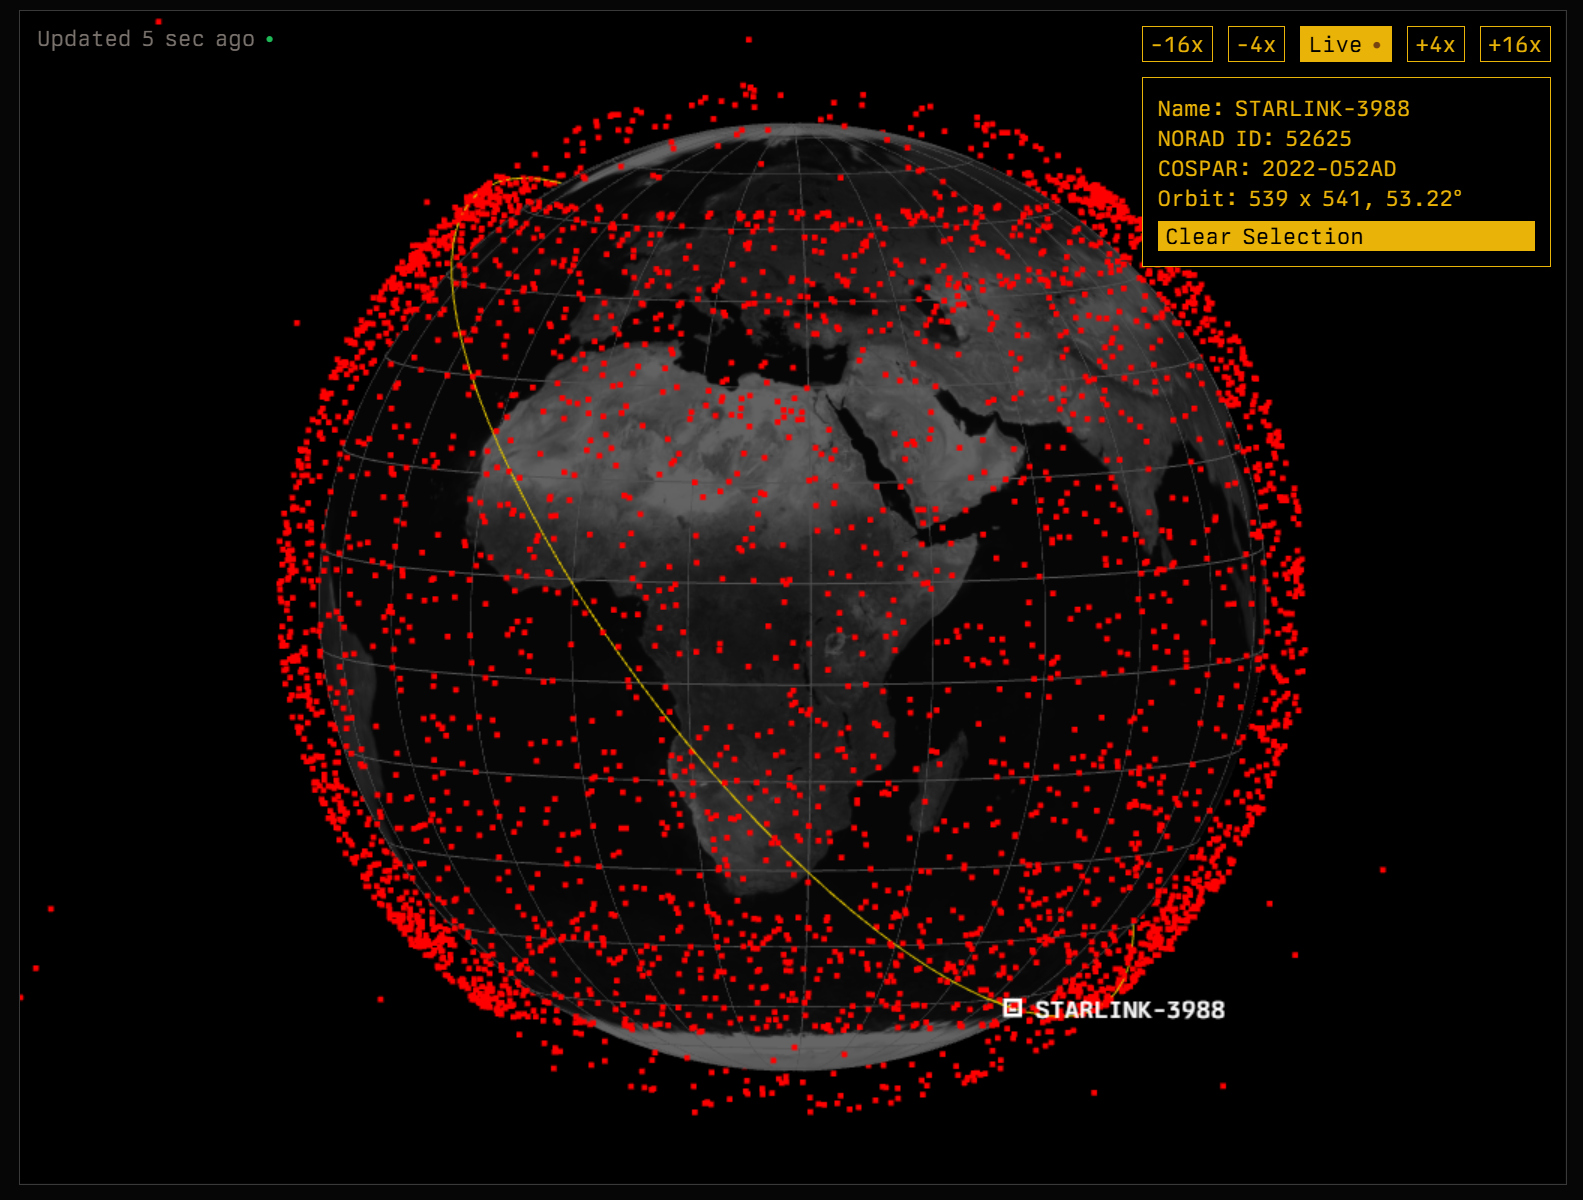
\includegraphics[width=\textwidth]{LaTeX/Figures/Starlink Constellation.png}
    \caption{Starlink constellation as of October 19th 2025, 16:59:33. Each red square represents an active satellite. Highlighted in yellow is the orbital track of selected satellite \textit{Starlink-3988}, with relevant orbital information displayed. The image is a screenshot from the Starlink Map website~\cite{starlinkmap.org}.}
    \label{fig:constellation}
\end{figure}

These satellites have already been used for several key applications, including enabling WiFi connectivity in commercial airlines and cruises, providing life-critical broadband in hurricane-ravaged coastal towns and earthquake-shaken regions, and facilitating allied command and control operations in the Russo-Ukrainian War. The constellation includes nearly 9,700 satellites (as of the writing of this report), and is visualised in Figure~\ref{fig:constellation}. Each unit is equipped with four beamforming, phased array antennas, each of which electronically steers the \SI{11.7}{\giga\hertz} collimated downlink signals in real time to a \SI{24}{\kilo\metre}-diameter ground coverage cell that can serve up to 8,000 simultaneous customers. Furthermore, the satellites communicate with one another via five on-board optical lasers at vacuum light-speed, enabling lower effective latencies between far-away cities compared to underwater cables. This is particularly relevant for applications in stock market trading, where saving a few milliseconds in latency can have a huge impact on the decision-making reactions to market fluctuations. To add to the list of groundbreaking engineering innovations that SpaceX developed for Starlink satellites, the orbital insertion procedure is entirely novel: the satellites are deployed in clusters of up to 23 units\footnote{For the larger v2 model, down from up to 60 units of the smaller v1/v1.5 model} at an altitude of roughly \SI{280}{\kilo\metre}, then their orbits are slowly raised to around \SI{550}{\kilo\metre} in two stages using Kripton gas ion thrusters\footnote{This is a more cost-efficient alternative to the customary option, Xenon gas}. This unusual manoeuvre leaves the satellites bunched up in characteristic lines for a long period of time before successful insertion, and these can be observed from the surface of the Earth as shown in Figure~\ref{}.

This project aims to investigate the orbit of an active, Earth-orbiting satellite through empirical observation and data collection.







\section{Data Collection}

\section{Estimate of Period and Angular Velocity}

\section{Estimate of Semi-Major Axis and Position Prediction}

\section{Estimate of Orbital Elements}

\section{Error Analysis}

\section{Conclusion}

\section{Visualisation}

\printbibliography

\end{document}
